\chapter{StockTwits Classified Sentiment and Stock Returns}

\section{Introduction}
\label{S:1}

Recent developments in artificial intelligence and the growing amount of alternative data have created new areas of research in finance. In particular, often coming from news, social media or annual reports, textual data is increasingly used in the literature. \citet{nikfarjam2010text} documents recent text mining approaches for stock market prediction. The pioneer work from \citet{antweiler2004all} computes a bullishness measure out of 1.5 million messages posted on Yahoo! Finance and Raging Bull and finds that stock messages help predict market volatility. Their results clearly reject the hypothesis that all that talk is just noise. They show that there is financially relevant information present. Growing from that, there are now two main sides of sentiment analysis literature studying the forecasting abilities of natural language processing (NLP hereafter): text mining of annual reports and sentiment analysis using social media. On one side, \citet{shirata2011extracting} and \citet{cecchini2010making} report that extracting phrases from annual reports may be an effective predictor of corporate bankruptcy. Similarly, \citet{loughran2011barron} identify phrases that might be red flags indicating questionable behavior. On the other side, \citet{renault2017intraday} builds an intraday investor sentiment indicator using messages and finds that the change in investor sentiment of the first half-hour of a trading day helps forecast the last half-hour market return of that trading day.

We conjecture that our investor sentiment measure can serve as a proxy of unobservable firm fundamentals. For instance, misaligned managerial and shareholder incentives are not easy to observe quantitatively in firm's annual reports (see \citet{nikolov2014agency}) but analysts may talk about them freely in bearish messages. This flow of data can be used throughout a period to improve forecasts (see \textit{nowcasting} in \citet{challet2013predicting}). \citet{tetlock2008more} uses Wall Street Journal stories to examine whether the usage of language is able to predict individual firms’ accounting earnings and stock returns. They find that some aspects of firms' fundamentals are hard-to-quantify, but investors may use linguistic media content to capture information and incorporate it into stock prices.

Most papers studying social media's predictive power use Twitter as their primary source of data. Twitter has the advantage of being used by a wide range of people across the world and a few influencers can attract attention of many investors. In 2013, Carl Icahn tweeted that following a meeting with Tim Cook (Apple CEO), he bought a large position in Apple and believed that the company is extremely undervalued. This bullish tweet caused the market capitalization of Apple to jump by \$12 billion. In 2019, JPMorgan has created the \textit{Volfefe Index} to track Donald Trump's tweets impact on the stock market. However, it is more difficult to disentangle noise from relevant tweets in Twitter than in other more focused social media. Results from \citet{Ghoshal} show that StockTwits is significantly more informative than Twitter data. This is not surprising as StockTwits is a finance-only social media whereas Twitter also captures irrelevant opinions on a wide range of non-finance related matters.

To the best of our knowledge, our paper is the first that compares predictive power of messages in general and around specific events. \citet{ranco2015effects} is likely the closest paper to our study. However, the finance-tailored data we use allow us to get higher contemporaneous correlations between stock returns and polarity. We also use much more messages (90 million versus 1 million) during a longer period (10 years versus 13 months). We also add contribution by looking at the predictive power of cumulative average abnormal polarity (CAAP hereafter). Our paper also contributes to the Efficient Market Hypothesis (EMH hereafter) literature by gauging how cumulative average abnormal returns (CAAR hereafter) and CAAP behave around sudden peaks of message activity. We collect 90 million messages published on StockTwits from mid-2010 to the end of March 2020. On this microblogging platform, users are invited to identify firms with their ticker when they share opinions. Another useful feature on the platform is the possibility to explicitly label their own messages as \textit{bearish} or \textit{bullish} when users post them. We believe that messages on the platform are reliable for several reasons. First, users have incentives to publish valuable information in order to maintain or increase mentions and/or retweets and thus have a greater share of voice in the forum (\citet{sprenger2014tweets}). In addition, market manipulations happen rarely because malicious users have incentives to post fake news only if they previously traded in the same direction than the news they are creating, which will only benefit them if they already have influence on the platform. Finally, SEC closely monitors large influencers to prevent any market abuse. 

The challenge in this context is to create a classifier that understands the vocabulary of the messages posted by the investors. For instance, ``bull" is an animal in everyday language but it is someone optimistic in the financial jargon. Work has already been done in this direction: \citet{loughran2011liability} creates a word list, which helps classify tone in a financial document. However, this might not be sufficient in the context of social media because messages posted present many typos, abbreviations and slang, so one needs to have an additional layer of data preprocessing. For instance, the word ``goooooood" would not be recognized by the model if it is not corrected into ``good" first. 

In this paper, we use a logistic regression on Term Frequency-Inverse Document Frequency (TFIDF hereafter) vectorized labeled messages to classify unlabeled messages in either bearish, bullish or neutral class. TFIDF is a weighting scheme gauging the importance of a word in a document (see \citet{erdemlioglu2017market}). As users are prone to post more bullish messages than bearish messages, a good classifier needs to take into account the unbalanced data. Without resampling, the classifier outputs classification scores biased towards the over-represented class. Because we are creating an artificial neutral class, we chose to not resample the data but rather optimally select classification score thresholds by maximizing F1 scores of two distinct classification algorithms: bullish versus non-bullish and bearish versus non-bearish. Then, we aggregate messages daily for every firm to compute sentiment polarity time series for individual firms and for the whole economy. 
%\todo{we should find a concise definition of polarity to be put in the abstract and introduction} \TODO{agree. what about something like : degree of bullishness observed on a given firm on a given day}
%Similarly, \citet{pang2002thumbs} suggests that ``there are certain words people tend to use to express strong sentiments, so that it might suffice to simply produce a list of such words by introspection and rely on them alone to classify the texts." 

We then use the daily volume of messages on a given firm to identify sudden peak of activity, indicating a firm event. Using abnormal polarity on each event date, we are able to classify events into three classes: bullish, neutral and bearish. We then compute cumulative average abnormal return and cumulative average abnormal polarity in a 41 days window centered at the identified event. We show that abnormal polarities have significantly higher predictive power than abnormal returns. On average, changes of polarity are associated with changes of contemporaneous return of the same sign; but this result does not hold against next-day return. However, when we focus on specific events, polarity has strong predictive power. It is also interesting to note that polarity tends to be biased towards recent past events. Finally, as robustness check, our event study on CAAR is similar to previous literature and is consistent with Fama’s theory.

The remainder of the paper is structured as follows. Section \ref{S:data} presents the data. Section \ref{S:classification} develops the NLP logistic classifier on TFIDF vectorization. Section \ref{S:polarity} explains our polarity measure. Section \ref{S:event studies} contains the results of the event studies. Section \ref{S:portfolios} shows the portfolio construction and Section \ref{S:conclusion} concludes.


\section{Data}
\label{S:data}

Data is coming from two sources: Compustat/CRSP for the stock prices, StockTwits for the investor sentiment. From the CRSP database, we extract daily stock prices (closing prices), daily volume of transactions and number of shares outstanding from 2010 to 2020 for all US and Canadian firms. Stock prices and number of shares are adjusted to account for any distribution (i.e. dividends, stock splits) so that a comparison can be made on an equivalent basis before and after the distribution. 

StockTwits is a large social network similar to Twitter but designed for investors and traders. Users register online and can post messages about any listed firm through the prefix \$ followed by the ticker of the firm. StockTwits was created in 2008 as an app built on the Twitter's API and later detached from Twitter to build a standalone social network. As of April 2019, it has over two million registered users and the number of messages posted is growing exponentially (see Figure \ref{fig:tweet_vol_daily}). StockTwits describes itself as ``the voice of social finance and the best way to find out what is happening right now in the markets and stocks you care about". In practice, it is effectively used by finance professionals to express their opinions on individual firms and the market as a whole. Since mid-2010, users also have the possibility to label their own messages as either \textit{bullish} or \textit{bearish}. This feature is very useful for researchers as even though many messages are unlabeled, it allows for sentiment classification using NLP techniques. The reasons of using StockTwits and not another social media is threefold. First, one of the main challenge in Natural Language Processing is the creation of an appropriate labeled vocabulary. \citet{loughran2011barron}) shows that it is essential to have a specific vocabulary to interpret finance documents (i.e many words have a different meaning in finance than in traditional English (e.g “bear trap”)). In addition to that, social media slang is an additional layer of language complexity. To this extent, the functionality to self-tag \textit{bullish} and \textit{bearish} messages that StockTwits implemented in 2012 is very valuable as it allows the creation of a specific labeled vocabulary out of labeled messages. We are not aware of any other social media platform in finance offering this functionality. Second, StockTwits is less noisy than Twitter because messages focus on finance and economics matters only. Third, extracting data out of StockTwits is easy because of its API. StockTwits' API is designed to query the database to download messages via JSON requests. Using a Python script, we extract all messages since the 10th of July 2009 until the 31st of March 2020 for a preset list of tickers coming from the Compustat database corresponding to all US and Canadian firms. This results in 90 million messages, which we download and store as JSON files. As one message may refer to several tickers, we consider a message with two or more tickers as one message for every ticker identified. We refer to the appendix for more information about this process.
 
 \begin{figure}
    \centering
    \includegraphics[width=0.75\textwidth]{tweet_vol_daily.JPG}
    \mycaption{Number of messages posted daily on StockTwits.}{}
    \label{fig:tweet_vol_daily}
\end{figure}

Every message comes with the following eight features: (1) the ticker discussed (2) the exact timestamp of the message, (3) a unique message identifier, (4) the body of the message, (5) the sentiment label (bearish, bullish, or none) entered by the user, (6) a unique identifier of the user who sent the message, (7) the number of messages published by the user who sent the message, and (8) the number of followers of the user who sent the message. Figure~\ref{screenshot} shows a screenshot of the StockTwits website as of 3rd March 2020, for a query on the AAPL\footnote{AAPL is the ticker for Apple.} ticker. The first message is labeled as bullish by the user ``satkaru", the two next are unlabeled messages that will be classified using a machine learning classifier, and the last message is labeled as bearish by the user ``Etrading''. 

\begin{figure*}[h]
\centering
\includegraphics[width=0.75\textwidth]{stocktwits_screeshot_3march2020.JPG}
\mycaption{Screenshot of StockTwits as of 3rd March 2020.}{The first message is labeled as bullish by the user ``satkaru", the two next are unlabeled messages that will be classified using a machine learning classifier and the last message is labeled as bearish by the user ``Etrading''.}
\label{screenshot}
\end{figure*}




Figure \ref{categrepartition-preclassif} shows the distribution of user-labeled and unlabeled messages. Overall, around 30 million messages are user-labeled and 60 million messages are unlabeled. Among the user-labeled messages we find five times more bullish than bearish ones. This ratio indicates that investors are on average optimistic about the market, which is consistent with findings in the literature, e.g., \citet{renault2017intraday}. Such class imbalance is a well-known issue in machine learning classification, which we address below. We will classify the unlabeled messages using a machine learning algorithm trained on the set of user-labeled messages. Since not every message contains substantial information, we believe that the sentiment classification should not be a bullish/bearish dichotomy. Hence, we allow for a neutral class to account for messages that do not take a clear stand.

\begin{figure*}[h]
\centering
        \begin{subfigure}[b]{0.75\textwidth}   
            \centering 
            \includegraphics[width=\textwidth]{preclassif.JPG}
        \end{subfigure}
        \mycaption{Number of user-labeled messages in each category.}{There are around 60 million unlabeled messages that we classify using the 30 million user-labeled bullish and bearish messages.} 
        \label{categrepartition-preclassif}
\end{figure*}



Figure \ref{fig:data-stocktwits1} shows a log-log histogram of the number of followers per user and a log-log histogram of the number of messages posted by users. As expected, there are few users with many followers (they can be seen as ``influencers"), and many users with a few followers. In addition, most users seem to post on average between 10 and 400 messages and a few post a lot more. 


\begin{figure*}[]
\centering
        \begin{subfigure}{0.75\textwidth}   
            \centering 
            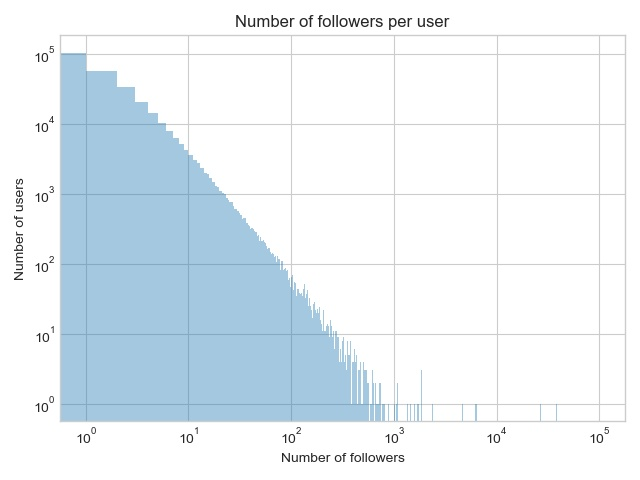
\includegraphics[width=\textwidth]{Followers.JPG}
        \end{subfigure}
        \quad
        \begin{subfigure}{0.75\textwidth}
            \centering
            \includegraphics[width=\textwidth]{Tweets.jpg}
        \end{subfigure}

        \mycaption{User summary statistics.}{Top graph is a log-log histogram of the number of followers per user and the bottom graph shows the log-log histogram of the number of messages posted by users.} 
        \label{fig:data-stocktwits1}
\end{figure*}


Figure \ref{fig:data-stocktwits2} shows the top 30 most discussed tickers on the platform. Of all tickers extracted, around 75\% are ordinary common share, 15\% are ETFs and the remaining 10\% are other types of securities. Not surprisingly, the S\&P index is the most discussed, followed by Apple and other big tickers. The messages about the 15 (30) biggest tickers represent 20\% (25\%) of the total number of messages, which indicates that users talk about a wide panel of tickers and not only big firms. The bottom graph shows a histogram of the number of messages per ticker. The x-axis is log-scaled because of extreme values, the distribution is highly skewed. 

\begin{figure*}[]
\centering
\begin{subfigure}{0.75\textwidth}  
            \centering 
            \includegraphics[width=\textwidth]{top30tickers.jpg}
        \end{subfigure}
        \quad
        \begin{subfigure}{0.75\textwidth}   
            \centering 
            \includegraphics[width=\textwidth]{LogTweetsPerFirm_3.jpg}
        \end{subfigure}
        \mycaption{Firm summary statistics.}{Top graph shows the top 30 most discussed tickers on the platform. SPY is the ticker of the S\&P and AAPL is the ticker for Apple. Bottom graph shows the distribution of the number of messages across tickers.} 
        \label{fig:data-stocktwits2}
\end{figure*}

Messages contain qualitative information, which needs to be transformed into quantitative data for the computer to understand. Thereto, we first apply the following preprocessing operations: an apostrophe handler, a contraction form handler (i.e. ``aren't" becomes ``are not"), tickers removal, stop words (i.e. ``a", ``the", ``of") removal\footnote{We follow \citet{renault2020sentiment} and \citet{saif2014stopwords} and use a restrictive list of stopwords to avoid accuracy decrease.}, users removal, lemmatization, URLs removal and a simple spell corrector dealing with more than two repeated characters (i.e. ``soooo goooood" becomes ``soo good"). Table \ref{tab:preprocess} shows five examples of messages before and after preprocessing.
 
One of the first steps in NLP is the tokenization : the way of slicing a piece of text in smaller units called tokens or terms. In financial lingo, some words only have meaning when associated with other words (i.e ``bad apple" or ``bear flag"). N-gram models allow accounting for words frequently occurring together with other words. The main hyperparameter in N-gram models is the size of the group of words considered : unigram is a term with only one word, bigram is a term with two consecutive words, etc. Bigger N-grams models increase dramatically the size of the vocabulary (i.e : the collection of all terms considered). We are able to control the size of the vocabulary by tuning a hyperparameter keeping only a given number of most frequent terms.  We chose to work with a vocabulary consisting of the one million most frequent unigrams, bigrams or trigrams. 

Figure \ref{wordclouds} represents the bullish and bearish word clouds. These correspond to the most frequent terms (up to 3-grams) in user-labeled bullish (bearish) messages relative to their total appearance. The size of the terms represent their importance in the cloud. In the bullish cloud, we see words such as ``bullish divergence", ``room to grow", ``lot potential" which are clearly bullish signals. In the bearish cloud, we find words such as ``recent resistance", ``short setup", ``bad apple" which indeed indicate bearish signals. These findings are reassuring in the sense that the content of the messages on the platform are consistent with their labels. The term ``aldox" in the bullish cloud caught our attention. After some research, it is an abbreviation for Aldoxorubicin, a drug against tumors and is associated with pharmaceutical messages where investors were very enthusiastic about it (example of related message: ``aldox is on the slide. have great faith this is truly world change"). That is why the term is appearing almost exclusively in bullish messages, hence in the bullish cloud.

On another note, most of the times messages are written by humans. It is however possible that some messages are generated by a robot (for instance to spread news or articles). In such cases, we define a neutral class that would absorb these messages if no substantial information is embedded in these messages. The term "long position open" present in the bearish cloud is an anomaly due to bearish user-labeled messages of intraday alerts such as “sell \$labd close labd long position. open labd short position. time: 14:53 ny price: \$13.64 zquant intraday alerts”. However, such anomalies are not an issue, a message “long position open” has a bullish probability of 0.91 and gets classify as bullish as it should. This is the case because when classifying a message, the score of the unigram “long” is much stronger than the score of the trigram “long position open”. From a linguistic point of view our approach is brute force. However, in turn, it works at a massive scale. Overall, the data quality is very good.


\begin{figure}
\begin{center}
    \includegraphics[width=0.75\textwidth]{Positive rate words.jpg}

    \vspace{1cm}

    \includegraphics[width=0.75\textwidth]{Negative rate words.jpg}
   \vspace{0.1cm}
    \mycaption{Bullish and bearish word clouds.}{Bullish word cloud (top), bearish word cloud (bottom). These correspond to the most frequent terms (up to 3-grams) in user-labeled bullish (bearish) messages relative to their total appearance. The size of the terms represent their importance in the cloud.}
    \label{wordclouds}
  \end{center}
\end{figure}


\newpage
\begin{table}[H]
\begin{tabular*}{\textwidth}{l@{\extracolsep{\fill}}ll}
\hline \multicolumn{2}{l}{Before preprocessing}                         \\   \hline \hline                                                                          
(1) & @CassandraTwit \$uvxy contango 3.5\%...still long. goooooood      \\
(2) & \$FRPT Take profits while you still can. \\
(3) &  \$UVXY \$tvix go time boys and girls. Holding overnight again                                                                                                                                        \\
 (4) & \$dnr Nice upgrade as company goes into its quiet period!      \\
 (5) & \$SPY market won't reverse again towards closing. Get put options. \\ 
 \hline                                                                                          
\end{tabular*}
\end{table}

\begin{table}[H]
\begin{tabular*}{\textwidth}{l@{\extracolsep{\fill}}ll}
\hline \multicolumn{2}{l}{After preprocessing}               \\   \hline \hline                                                                       
(1) & contango still long good            \\
(2) & take profit while you still can \\
(3) & go time boy and girl hold overnight again                                                                  \\
(4) & nice upgrade as company go into its quiet period     \\ 
(5) & market will not reverse again towards closing get put options \\ \hline                                          
\end{tabular*}
\mycaption{Preprocessing of five sample messages.}{Preprocessing operations include: punctuation removal, lower casing, apostrophe handling, contraction form handling (i.e. ``won't" becomes ``will not"), tickers removal, users removal, URLs removal, parsing and a simple spell corrector dealing with more than two repeated characters (i.e. ``goooood" becomes ``good")}
\label{tab:preprocess}
\end{table}

\section{Sentiment classification}\label{S:classification}

Since mid-2010, StockTwits users have the choice to label their own messages as either \textit{bearish} or \textit{bullish} or to leave it unlabeled. Unlabeled messages are tricky to deal with because the user either deliberately chose to leave the message neutral by not labeling it or forgot to click on a label. Figure \ref{fig:ts_neutral_vs_uncl} shows the proportions of user-labeled messages in each category across time. In the early years of the platform, most messages are unlabeled, presumably because users were not familiar with the sentiment label yet. Albeit the proportion of unlabeled messages monotonically declines over the years, almost 60\% of the more recent messages are still unlabeled. We believe that by far not all unlabeled messages reflect neutral opinions. Figure \ref{fig:postclassif_acrosstime} shows that a lot of unlabeled messages get classified in either bullish or bearish messages, hence these unlabeled messages had indeed valuable information that we are now able to capture. 

\begin{figure}[h]
    \centering
    \includegraphics[width=0.75\textwidth]{preclassif_acrosstime.JPG}
    \mycaption{Proportions of user-labeled messages in each category}{Proportions of user-labeled messages in each category: bullish (green), bearish (red), and unlabeled (gray). Proportions are aggregated monthly.}
    \label{fig:ts_neutral_vs_uncl}
\end{figure}


As one of the goal of this paper is to build an accurate time-series sentiment measure for individual firms, it motivates the use of Natural Language Processing to classify all unlabeled messages in either bullish, neutral or bearish class.

To classify unlabeled messages, we use a logistic regression of the labels on TFIDF transformed user-labeled messages, as in \citet{nlp1} and \citet{classifq}. TFIDF stands for Term Frequency-Inverse Document Frequency and is a widely used method to transform a text, in our case a message $m$, into a numerical vector, $TFIDF_m$. The dimension of this vector is equal to the size of the vocabulary (the collection of all terms across all messages). The components of the vector encode the importance of the corresponding terms $t$ in the message $m$, as formally defined by $TFIDF_{m,t} = TF_{m,t} \cdot IDF_t$. The first factor measures how frequently term $t$ appears in the message,
\[ TF_{m,t} =\dfrac{\sum_{i=1}^{N_m} \textbf{1}_{t=t_{m,i}}}{N_m},\]
where $N_m$ denotes the number of terms $t_{m,i}$ in message $m$. The second factor measures how important term $t$ is to the message,
\[ IDF_t = \log \big(\dfrac{V}{\sum_{j=1}^{V} \textbf{1}_{t \in m_j}}\big),\]
where $V$ denotes the total number of messages $m_j$. A term $t$ appearing in many documents (such as ``the", ``is", ``of") is likely to have low information content, hence a low $IDF_t$. 

As seen in Figure \ref{categrepartition-preclassif}, user-labeled messages exhibit five times more bullish messages than bearish messages. Such an imbalance is a well-known issue in machine learning classification and needs to be dealt with to avoid biases towards the over-represented class (see \citet{chawla2004special}). To tackle class imbalance, the most common technique is to randomly oversample the minority class, which consists of repeating some samples of the minority class and balance the number of samples between classes in the data. We follow a different approach. In addition to bullish and bearish classes, we define an artificial neutral sentiment class as it is possible that some users are not expressing any opinion and sometimes post finance-irrelevant messages. To do so, we optimally select classification score thresholds and eliminate the class imbalance bias at the same time.

Performance measures widely used in machine learning classification are precision, recall, F1 score and accuracy. The first step is to define a class as the positive class. Instances (messages) are then divided into true positives TP (predicted positive, actual positive), false positives FP (predicted positive, actual negative), true negatives TN (predicted negative, actual negative), and false negatives FN (predicted negative, actual positive). Precision $PRE=\dfrac{TP}{TP+FP}$ is the proportion of true positives among the predicted positives. Recall $REC = \dfrac{TP}{TP+FN}$ is the proportion of true positives among the actual positives. The precision-recall trade-off is captured by the F1 score, $\dfrac{2 \cdot PRE \cdot REC}{PRE + REC}$, the harmonic mean of precision and recall. Accuracy $ACC = \dfrac{TP+TN}{TP+TN+FP+FN}$ is the fraction of correct predictions regardless of the label.
 

We use 80\% of the user-labeled (bearish and bullish) messages as a training set and keep 20\% as a test set, then we run two binary classifiers. The first (second) classifier sets bullish (bearish) as positive and non-bullish (non-bearish) as negative class. Every message then falls into the following set of labels: \{(non-bullish, bearish), (bullish, bearish), (non-bullish, non-bearish), (bullish, non-bearish)\}. For the two outer cases the two algorithms agree and the final classification is defined to be bearish (non-bullish, bearish) or bullish (bullish, non-bearish), respectively. For the two inner cases, (bullish, bearish) and (non-bullish, non-bearish), the two algorithms disagree, so that the final classification is defined to be neutral. Formally, every message $m$ is then mapped on either

\[ m\mapsto \begin{cases} \text{(non-bullish, bearish)} & =: \text{bearish} \\ \text{(bullish, bearish)}& =: \text{neutral} \\ \text{(non-bullish, non-bearish)}& =: \text{neutral} \\ \text{(bullish, non-bearish)} &=: \text{bullish.} \end{cases}\] 

Precision, recall, and F1 scores of the two algorithms differ because they depend on which class is defined as the positive one. To select optimal classification thresholds, we maximize the F1 score of either algorithm. The green (red) line in Figure \ref{fig:optimal_thresholds} is the F1 score for the bullish versus non-bullish (bearish versus non-bearish) classification, respectively. Circles indicate the maximal F1 scores, along with the corresponding classification score thresholds, 0.50 and 0.72, respectively. 

\begin{figure}[h]
    \centering
    \includegraphics[width=0.75\textwidth]{optimal thresholds.JPG}
    \mycaption{Optimal classification thresholds.}{The green (red) line is the F1 score for the bullish versus non-bullish (bearish versus non-bearish) classification, respectively. Circles indicate the maximal F1 scores, along with the corresponding classification score thresholds.}
    \label{fig:optimal_thresholds}
\end{figure}


If the classification score of a message is bigger (smaller) than 0.72 (0.50), then both classifiers agree on the sentiment and the message is classified as bullish (bearish), respectively. If the classification score is between 0.50 and 0.72, the classifiers disagree, (bullish, bearish), and we consider the message as neutral. Finally, we overwrite the sentiment of a message predicted by the classifier by the user-labeled sentiment whenever the latter is available. Research in sentiment classification shows that human annotators tend to agree about 80 to 85\% of the time when evaluating the sentiment of a document (see e.g. \citet{wilson2005recognizing} and \citet{chen2020large}). This usually represents the accuracy that a sentiment classifier should meet or beat. The accuracy in the test set of our combined classifier is 86\%.


Figure \ref{fig:postclassif_acrosstime} shows the proportions of classified messages in each category. Percentages of bearish (sum of labeled and classified as bearish) and bullish (sum of labeled and classified as bearish) messages are stable over time, suggesting that our classification method is robust. Even if most messages were not user-labeled in the early years of the platform, as seen in Figure \ref{fig:ts_neutral_vs_uncl}, we are now able to classify the sentiment of most messages posted in this period. Consistent with the over-representation of bullish messages observed in the user-labeled messages in Figure \ref{categrepartition-preclassif}, there are many more messages classified as bullish than bearish. Typical messages classified as bullish are messages such as “buy buy” or “hope the pump come soon” whereas typical bearish messages are messages such as “sell everything” or “start short position here”. Neutral messages are either empty, irrelevant to finance (e.g. “political posturing friend”\footnote{This is a reply to the following message : "honestly, how dumb can you be to believe that china was going to buy significant amount of agricultural products after the breakdown in trade talks. even if they buy it will be just a little bit and not significant"}) or ambiguous (e.g. “lol wow”).
 

\begin{figure}[h]
    \centering
    \includegraphics[width=0.75\textwidth]{postclassif_acrosstime3.JPG}
    \mycaption{Proportions of classified messages in each category}{Bullish (light green predicted, green user-labeled), bearish (light red predicted, red user-labeled), and neutral (gray). Proportions are aggregated monthly.}
    \label{fig:postclassif_acrosstime}
\end{figure}


\section{Polarity}\label{S:polarity}

To build sentiment measures for individual firms and the whole market on a given day, we count the sentiments in the messages. To match the timeline on which close-to-close stock returns are computed and to avoid forward-looking bias, we aggregate messages on a close-to-close manner. That is, polarity on day $t$ is computed with messages posted from 4:00 pm on day $t-1$ to 4:00 pm on day $t$. As stock returns are not computed outside of business days, we shift messages posted outside of business days to the next business day available, then remove any non-business day from our sample. We denote by $C_{i,t,j}$ the sentiment of the $j$th message about firm $i$ on day $t$. It is set to 1, 0, or -1 for bullish, neutral, or bearish, respectively. We follow \citet{ranco2015effects} and define the polarity of firm $i$ as
\[    P_{i,t} = \dfrac{\sum_{j=1}^{V_{i,t}} (\textbf{1}_{C_{i,t,j} = 1} - \textbf{1}_{C_{i,t,j} = -1})}{\sum_{j=1}^{V_{i,t}} (\textbf{1}_{C_{i,t,j} = 1} + \textbf{1}_{C_{i,t,j} = -1})},\]
where $V_{i,t}$ denotes the number of messages about firm $i$ on day $t$.\footnote{If $V_{i,t}=0$ then we set $P_{i,t} =0$.}

As an aggregate measure, we define the polarity for the whole market as a weighted average over all firms 
\begin{equation*}
\label{marketpoleq}
    P_t^M = \dfrac{\sum_{i} V_{i,t} \cdot P_{i,t}}{V^M_t} ,
\end{equation*}
where $V^M_t = \sum_{i} V_{i,t}$ denotes the number of messages on day $t$.

Figure \ref{fig:marketpolspy} shows a scatter plot of the market polarity $P_{t}^M$ versus the polarity of the SPY\footnote{SPY is an ETF tracking the S\&P500 return. It is the largest ETF in the world.}. We do not expect the market polarity to be the SPY polarity because the stock universe is not the same (market polarity contains stocks that are not necessarily in the S\&P500 and vice versa). The slope coefficient of the regression line is statistically significantly positive and the contemporaneous Pearson correlation coefficient is 0.53, suggesting that the market polarity is an accurate measure of the aggregated sentiment of the market. Also, consistent with Figure \ref{fig:postclassif_acrosstime}, SPY and market polarities are bullish-biased.

\begin{figure}[h]
    \centering
    \includegraphics[width=0.75\textwidth]{spy_vs_marketpol.JPG}
    \mycaption{Market polarity versus the SPY polarity.}{Market polarity on the y-axis versus the polarity of the SPY on the x-axis. The red line shows the linear regression line and coefficients.}
    \label{fig:marketpolspy}
\end{figure}

At this point, for stationary reasons\footnote{Computing the polarity ratio with few daily observations would lead to a spiky time series.}, we compute the median of daily message volume for each ticker and exclude from our sample tickers that have less than a median of 50 daily messages. Our final sample contains 19 tickers. We refer to the appendix for the list of tickers covered as well as more information about the trimming process. 

To understand how polarity is related to investor sentiment, we run two linear regressions of contemporaneous daily returns on polarity and 5-days Cumulative Abnormal Polarity :
\begin{align*}
    R_{i,t} &= \alpha + \beta \cdot P_{i,t} + \epsilon_{i,t}, \\
    R_{i,t} &= \alpha + \beta \cdot CAP_{i,5} + \epsilon_{i,t}. 
\end{align*}
Table \ref{regpolret} shows that $\beta$ is positive and significant for both regressions. This indicates that polarity is a good proxy for the sentiment of investors. Further supporting evidence is given by the correlation between polarity and contemporaneous stock returns at the firm level. Figure \ref{fig:ts} shows the time series during 2019 for the top 6 most discussed tickers. In our entire panel of firms, correlations are always positive and range between 0.1 and 0.3.

\begin{table}[]
\centering
\begin{tabular}{l|c|c|c|c|c}
                     & $R_{i,t}$ & $R_{i,t}$   & $R_{i,t+1}$ & $R_{i,t+1}$        \\ \toprule 
Constant             & -0.0047*** & -7.92e-05   & -0.0002    & 7e-06         \\
                     & (0.000)    & (9.81e-05)  & (0.000)    & (9e-05)       \\
$P_{i,t}$           & 0.009***   &               & 0.0003     &               \\
                     & (0.000)    &               & (0.000)    &               \\
$CAP_{i,5}$         &            & 0.0007***     &            & -0.0002       \\
                     &            & (0.000)       &            & (0.000)       \\ \bottomrule
$R^2$                & 0.012      & 0.000         & 0.000      & 0.000              \\
No. Obs.             & 34100      & 34024         & 34100      & 34024             
\end{tabular}
\mycaption{Linear regressions }{Results from linear regressions of contemporaneous and next period stock returns on polarity. Stock returns are trimmed at the 5\% percentile on both sides. Standard errors are reported in parentheses. Statistical significance at the 99\%, 95\%, and 90\% level is indicated with ***, **, *, respectively.}
\label{regpolret}
\end{table}


\begin{figure*}[]
        \centering
        \begin{subfigure}[b]{0.48\textwidth}
            \centering
            \includegraphics[width=\textwidth]{ts_pol_ret_aapl.JPG}
        \end{subfigure}
        \quad
        \begin{subfigure}[b]{0.48\textwidth}  
            \centering 
            \includegraphics[width=\textwidth]{ts_pol_ret_amzn.JPG}
        \end{subfigure}
        \vskip\baselineskip
        \begin{subfigure}[b]{0.48\textwidth}   
            \centering 
            \includegraphics[width=\textwidth]{ts_pol_ret_tsla.JPG}
        \end{subfigure}
        \quad
        \begin{subfigure}[b]{0.48\textwidth}   
            \centering 
            \includegraphics[width=\textwidth]{ts_pol_ret_spy.JPG}
        \end{subfigure}
                \vskip\baselineskip
        \begin{subfigure}[b]{0.48\textwidth}   
            \centering 
            \includegraphics[width=\textwidth]{ts_pol_ret_amd.JPG}
        \end{subfigure}
        \quad
        \begin{subfigure}[b]{0.48\textwidth}   
            \centering 
            \includegraphics[width=\textwidth]{ts_pol_ret_fb.JPG}
        \end{subfigure}
        \mycaption{Time series of daily polarity}{Time series of daily polarity  (red - left axis) and daily stock returns (blue - right axis) since 1st of January 2019 for the top 6 most discussed tickers. Pearson correlation between the two time series is shown in the title.} 
        \label{fig:ts}
    \end{figure*}

We also run two linear regressions of next day returns on polarity and 5-days Cumulative Abnormal Polarity :
\begin{align*}
    R_{i,t+1} &= \alpha + \beta \cdot P_{i,t} + \epsilon_{i,t}, \\
    R_{i,t+1} &= \alpha + \beta \cdot CAP_{i,5} + \epsilon_{i,t}. \\
\end{align*}
Table \ref{regpolret} reveals that polarity has no predictive power for next day stock returns unconditionally. However, the next section depicts how polarity still has embedded information around specific events.

\section{Event studies}\label{S:event studies}

Event studies constitute a statistical method widely used in financial econometrics. In general, they are used to measure the effect of events on the market value of firms. Well known applications of event studies include the testing of various forms of the efficient market hypothesis (EMH) (see \citet{fama1969} and \citet{fama1991efficient}). What's more, as described in \citet{mackinlay1997event}, event studies can also be applied with little modification to other variables than stock returns. 

To design an event study, the first step is to define events of interest and the \textit{event window} over which a variable will be examined. Adhering to common practice, we choose the event window expanded from 20 business days before the event to 20 business days after the event. The \textit{estimation window} is used to estimate the parameters of the market model. A common choice is a one-year window ending 20 days before the event. Figure \ref{fig:timeline} shows the corresponding timeline. 

\begin{figure}[h]
    \centering
    \includegraphics[width=0.75\textwidth]{timeline.JPG}
    \mycaption{Timeline of our event studies.}{$\tau$ is an event date, the event window has 41 business days centered around the event date and the estimation window is a one-year rolling period prior the event.}
    \label{fig:timeline}
\end{figure}

Then, event studies require the distinction between a normal and an abnormal measure. The normal measure is defined as the expected measure conditioning on the event not taking place. In other words, we need an expectation of the variable of interest that would have been measured if the event never existed. The abnormal measure is defined as the measure minus the normal measure. Formally, let $X_{i,t}$ be a measure of interest (i.e. stock return, polarity, ...), $AX_{i,t}$ be the abnormal measure and $E(X_{i,t}|Z_{i,t})$ the normal measure with $Z_{i,t}$ being the conditional information for the normal measure model. We have: 
\[     AX_{i,t} = X_{i,t} - E(X_{i,t}|Z_{i,t}).\]

The normal measure $E(X_{i,t}|Z_{i,t})$ is usually computed using either a constant mean model or a market model. Constant mean models use $E(X_{i,t}|Z_{i,t}) = \mu$ where $\mu$ is the mean of the measure during the estimation window. We chose to work with a market model but all following results hold with the constant mean model as well. As stated in \citet{mackinlay1997event}, the variance of the abnormal measure is not reduced a lot by choosing a more sophisticated model, hence the event study is not sensitive to the choice of the normal model. 
The market model we are using is defined as the following: 
\begin{equation*}\label{eq_mm}
    X_{i,t} = \alpha_i + \beta_i \cdot X_{t}^M + \epsilon_{i,t},
\end{equation*}
with $E(\epsilon_{i,t}) = 0$, $V(\epsilon_{i,t}) = \sigma_{\epsilon}^2$ and $X_{t}^M$ the measure of the whole market. We estimate the parameters of the market model in a one-year rolling estimation window. To avoid overlaps between estimation windows and events, we remove any event day from the estimation windows. This ensures that large event returns do not influence the parameters of the normal measure.

\subsection{Events}
We define an event as an unusual high number of daily messages for a particular firm. We conjecture that a sudden peak in StockTwits message volume indicates that an important firm event is happening on the day of the peak. As a robustness check, we show in Figure \ref{fig:actvol} that increases (decreases) in number of message volume are positively associated with increases (decreases) in contemporaneous weekly volume of stock transactions. These co-movements mean that investors not only post about these stocks but also trade them simultaneously, adjusting their portfolios. This indicates that the message volume peaks is a good proxy to identify event dates as there is no lag between message activity and trades.

\begin{figure}
    \centering
    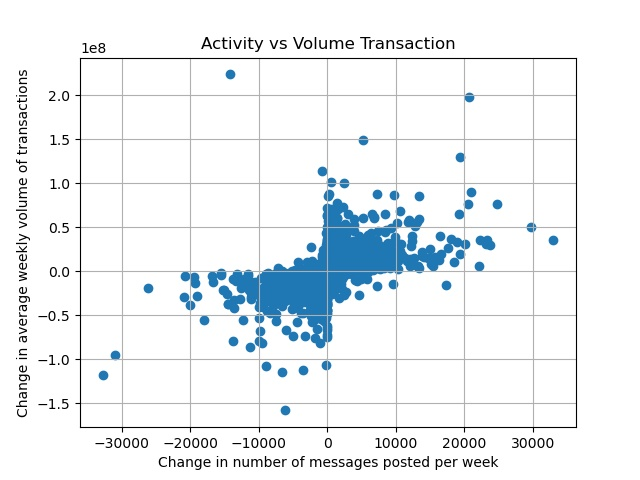
\includegraphics[width=0.75\textwidth]{activity-volume.jpg}
    \mycaption{Volume of transactions and message activity.}{Changes in weekly volume of transactions on the y-axis versus changes in message activity on the x-axis. Activity is measured in weekly messages posted per firm.}
    \label{fig:actvol}
\end{figure}

To measure unusual activity peaks, we use the market model (\ref{eq_mm}) on a one-year rolling estimation window and regress the daily relative change of message volume of individual firms $\dfrac{\Delta V_{i,t}}{V_{i,t-1}}$ on the daily relative change of total message volume $\dfrac{\Delta V_t^M}{V_{t-1}^M}$. Formally,
\[     \dfrac{\Delta V_{i,t}}{V_{i,t-1}} = \alpha_i^V + \beta_i^V \cdot \dfrac{\Delta V_t^M}{V_{t-1}^M} + \epsilon_{i,t}.\]
We can then compute the abnormal volume of messages for firm i as : 
\[     AV_{i,t} = \dfrac{\Delta V_{i,t}}{V_{i,t-1}} - \hat{\alpha}_i^V - \hat{\beta}_i^V \cdot \dfrac{\Delta V_t^M}{V_{t-1}^M}. \]
We define an event for ticker $i$ as a day $t$ where the standardized abnormal volume exceeds 2, 
\[   \dfrac{AV_{i,t} - \mu_{AV_i}}{\sigma_{AV_i}} > 2.\]

%To measure unusual activity peaks, we use the time series of individual firms message volume and identify days where the volume exceeds five times its rolling one-month median. Formally, the event dates for firm $i$ are the days $e$ such that:
%\begin{equation}
%    e = \{d : V_d > 5 \cdot V_m(d) \}
%\end{equation}
%where $V_d$ is the message volume on day d for firm i and $V_m(d)$ is the rolling one-month volume median at day d for firm i. 




Then, we define the type of the event as either bullish, neutral or bearish. We use the abnormal polarity $AP_{i,t}$ of the event date to assess how on average investors perceive the event. Figure \ref{fig:abnpol_all} shows the distribution of abnormal polarities. We chose to use the one-third (-0.03) and two-third percentile (0.07) of the distribution of abnormal polarities as thresholds for the type of the event. Conditionally on the existence of an event for firm $i$ at day $t$, we have:

\[     Type_{i,t}= \begin{cases}
      Bullish  & \text{if}\ \ AP_{i,t}> 0.07, \\
      Neutral  & \text{if}\ \ AP_{i,t} \in [-0.03, 0.07], \\
      Bearish  & \text{if}\ \ AP_{i,t} < -0.03. \\
\end{cases} \]


\begin{figure}[h]
    \centering
    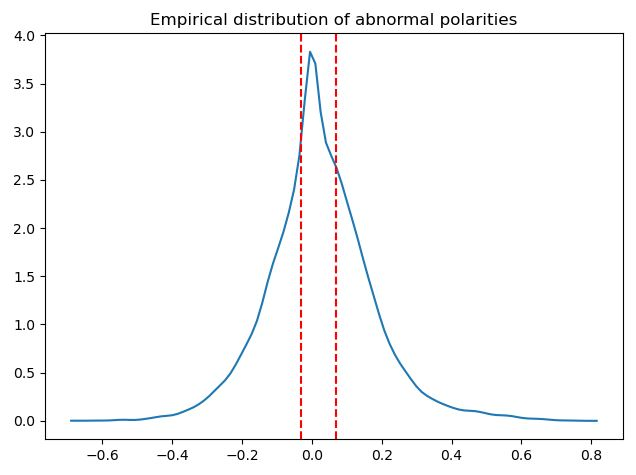
\includegraphics[width=0.75\textwidth]{abnpol_distr_all.JPG}
    \mycaption{Empirical distribution of abnormal polarities.}{Red dashed lines show the one-third and two-third percentiles.}
    \label{fig:abnpol_all}
\end{figure}


As an illustration, Figure \ref{fig:activityaapl} shows for Apple the time-serie of message volume and the bullish, neutral and bearish events identified as green up-triangles, gray circles and red down-triangles, respectively. Between 2011 and 2020, our algorithm identified 73 events for Apple. Interestingly, our methodology allows us to capture more than earning announcements : about half of these events correspond to earning announcements, but some also correspond to Apple \textit{Keynotes}\footnote{Keynotes are presentations that Apple gives to the press, often presenting new products.} or even CEO letters addressed to investors. Across 19 tickers, we identify 1131 events distributed across the three categories : 454 bullish events, 294 neutral events and 383 bearish events. This coverage is on par with previous studies (i.e: \citet{mackinlay1997event} has 30 firms and 600 events) Figure \ref{fig:events} shows the identified events and their types across the years.
%Table \ref{tab:aaplevent} shows all events for Apple and their associated types. 

\begin{figure}[]
    \centering
    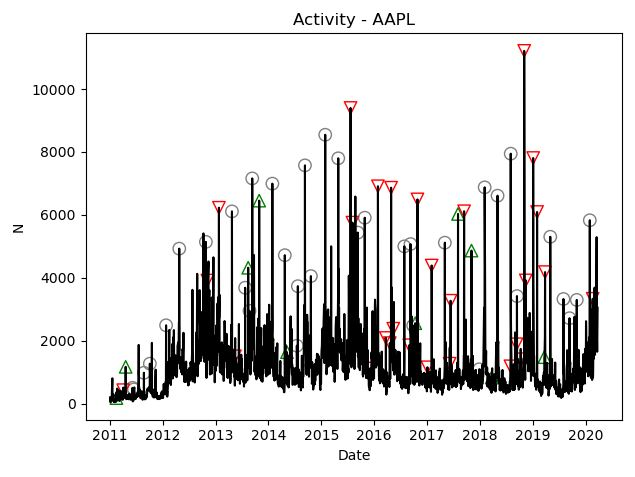
\includegraphics[width=0.75\textwidth]{activity_aapl.JPG}
    \mycaption{Daily message volume for Apple.}{Events are days with an unusual high number of messages. Green upper-triangles show bullish events, gray circles are neutral events and red down-triangles represent bearish events.}
    \label{fig:activityaapl}
\end{figure}

%\begin{table}[]
%\caption{Identified event dates and associated description for Apple between %2013 and 2020.}
%\centering
%\begin{tabular}{|l|l|}
%\toprule
%Date         & Description\\
%\bottomrule
%2013-10-28  & Earnings announcement\\
%2014-04-23  & Earnings announcement\\
%2014-09-09  & Keynote \\
%2015-10-27  & Earnings announcement\\
%2016-01-26  & Earnings announcement\\
%2016-07-26  & Earnings announcement\\
%2016-09-07  & Keynote \\
%2016-10-25  & Earnings announcement\\
%2017-01-31  & Earnings announcement\\
%2017-05-02  & Earnings announcement \\
%2017-08-01  & Earnings announcement \\
%2017-08-02  & Earnings announcement \\
%2017-09-12  & Keynote \\
%2017-11-02  & Earnings announcement\\
%2018-05-01  & Earnings announcement\\
%2018-07-31  & Earnings announcement\\
%2018-08-01  & First company to reach \$1 trillion\\
%2018-11-01  & Earnings announcement\\
%2019-01-02  & CEO Letter to investors\\
%2019-01-29  & Earnings announcement\\
%2019-03-25  & Keynote \\
%2019-04-30  & Earnings announcement\\
%2019-07-30  & Earnings announcement\\
%2019-09-10  & Keynote\\
%\bottomrule
%\end{tabular}
%\label{tab:aaplevent}
%\end{table}

\begin{figure}[]
    \centering
    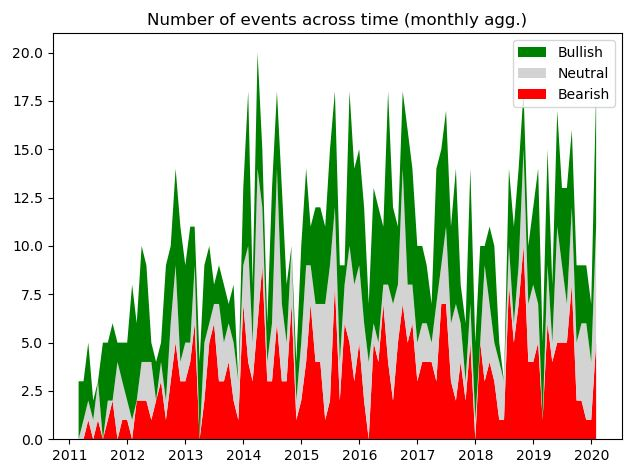
\includegraphics[width=0.75\textwidth]{events_across_time.JPG}
    \caption{Number of events in each category across time. Numbers are aggregated monthly.}
    \label{fig:events}
\end{figure}

\subsection{CAAR and CAAP}
We estimate the parameters for the market models using OLS, as it is a consistent and efficient estimator under general conditions.\footnote{An interested reader can refer to \citet{mackinlay1997event} for more details} 

\subsubsection{Abnormal Returns}
Given the market models parameters $\hat{\alpha_i}^R$ and $\hat{\beta_i}^R$ estimated in \eqref{eq_mm}, the abnormal return is
\[     AR_{i,t} = R_{i,t} - \hat{\alpha_i}^R - \hat{\beta_i}^R \cdot R_t^M,\]
with $R_t^M$ being the market return. Then, we can compute the cumulative abnormal returns (CAR) around a firm $i$ event $\tau$ as:
\[    CAR_i(\tau,t) = \sum_{s=- 20}^{t} AR_{i,\tau + s},\]
and finally get the cumulative average abnormal returns (CAAR) across the N events as:
\[     CAAR(t) = \dfrac{1}{N} \sum_{j=1}^N CAR_{i_j}(\tau_j,t).\]
Variance of CAR is computed following \citet{mackinlay1997event} as :
\[     var(CAR(\tau,t)) = \dfrac{1}{N^2} \sum_{i=1}^N (CAR_i(\tau,t) - CAAR(t))^2.\]

Figure \ref{fig:ES_CAAR_MM} shows the CAAR around the events identified. This plot is consistent with \citet{mackinlay1997event}. It shows that CAAR related to bearish (bullish) events displays a downward (upward) jump at the event date respectively, and then the jumps are followed by a stable CAAR during the 20 days period after an event. Interestingly, there is a systematic (small) shift in the CAAR already 1 day before an event. The CAAR related to the neutral events exhibits a slight upward shift around the event date but it fades away after a few days. The CAAR related to bearish events shifts already a few days before the event but this shift is not statistically significant. Additionally, as we see in the top-left plot of Figure \ref{fig:boxplotcaar}, box plots are not shifted, indicating that the conditional distributions of the CAR are not statistically different from each other. Mann-Whitney U-test (Table \ref{utest_res}) shows that 5 days before an event, the median of the CAR distribution of the bullish events is neither statistically different from the median of the neutral nor the bearish events.

\begin{figure}[h]
    \centering
    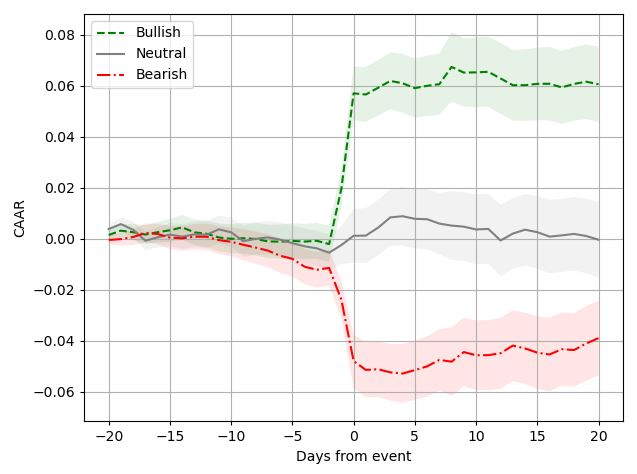
\includegraphics[width=0.75\textwidth]{caar.JPG}
    \mycaption{Cumulative average abnormal returns around identified events.}{CAAR related to bearish, neutral and bullish events are displayed with the red, gray and green line, respectively. Areas around lines show confidence intervals at the 95\% level.}
    \label{fig:ES_CAAR_MM}
\end{figure}

\subsubsection{Abnormal Polarity}
Similar to the subsection above, given the market models parameters $\hat{\alpha_i}^P$ and $\hat{\beta_i}^P$ estimated in \eqref{eq_mm}, the abnormal polarity is
\[    AP_{i,t} = P_{i,t} - \hat{\alpha_i}^P - \hat{\beta_i}^P \cdot P_t^M,\]
with $P_t^M$ being the market polarity computed in \eqref{marketpoleq}. Then, we can compute the cumulative abnormal polarity (CAP) and cumulative average abnormal polarity (CAAP) from $\tau - 20$ to $t \le \tau + 20$ as:

\begin{align*}
    CAP_i(\tau,t) &= \sum_{s=- 20}^{t} AP_{i,s+\tau}, \\
    CAAP(t) &= \dfrac{1}{N} \sum_{j=1}^N CAP_{i_j}(\tau_j,t).
\end{align*}

Figure \ref{fig:ES_cum_abn_pol_MM} shows the CAAP around the events identified. The main findings about polarity are twofold. First, conversely to CAAR, CAAP for bullish and bearish events are not constant after the event date, suggesting that users' sentiment about a firm tend to be biased towards recent past events. This can be explained by the fact that users might still post bullish or bearish messages about an event even several days after the event happening, even though the return had already adjusted. Second, and more interestingly, it looks like the CAAP for bullish and bearish events shift several days earlier than the CAAR. This would indicate that the users are on average able to anticipate a future bullish (bearish) event and post positively (negatively) about the firm days before the rise in CAAR. Figure \ref{fig:boxplotcaar} illustrates this striking result with box plots (see \citet{boxplot1} and \citet{boxplot2}) showing the distribution of the CAR and CAP. The line inside a box shows the median while the edges of each box represent the 25\% and 75\% quantile of the distribution. From above the edges of a box, a distance of 1.5 times the interquartile range is measured and a whisker is drawn up to the largest and lowest observed point from the data that falls within this distance.\footnote{Interquartile range is equal to the third quartile minus the first quartile.} The three plots on the left (right) show the boxplots for the CAR (CAP) 5 days before an event, on event date, and 5 days after the event, respectively. To show statistical significance, we use the Mann-Whitney U-test (see \citet{utest} and \citet{sheskin}) on every plot to assess whether the three samples (bullish, neutral and bearish) represent populations with different median values.\footnote{This interpretation only holds under stringent assumptions on the populations, namely that the two population distributions are equal up to a shift.}  Under the null hypothesis, the three samples represent distributions with equal medians.
 Let $\theta_i$ be the median of the distribution i. Formally, we test $H_0 : \theta_{bullish} = \theta_{neutral}$ against $H_1 : \theta_{bullish} > \theta_{neutral}$ and $H_0 : \theta_{neutral} = \theta_{bearish}$ against $H_1 : \theta_{neutral} > \theta_{bearish}$ 5 days before an event, on event date and 5 days after an event. We define U as the Mann-Whitney test statistic, Z as the normal approximation of the Mann-Whitney test statistic for large sample sizes, $n_1$ and $n_2$ as the sample sizes. We refer to \citet{sheskin} for the test statistic computation.
Table \ref{utest_res} shows U-test estimates for pairwise comparisons. The null is rejected in every case except for CAR at $t-5$. 5 days before the event, the boxes of the CAR between bullish, neutral and bearish events are on the same level, suggesting no predictive power of abnormal returns, consistent with the EMH. However, the boxes showing the CAP 5 days before the event are already shifted, meaning that conditionally on an event happening, investors are able on average to anticipate correctly the type of this event. On the event date, the boxes of the CAR shift as the abnormal returns jump for both bullish and bearish events, consistent again with the EMH. Finally, 5 days after the event, the distributions of the CAR are very similar to the distributions on the event dates. Again, this is consistent with the EMH as the abnormal returns adjusted quickly on event date and all information is now embedded in the prices. The distribution of the CAP 5 days after the event continued to shift compared to the event date, as people continue to post about recent past events.
% \TODO{maybe this part of the short story about EMH, which we should provide earlier, at the beginning of the event study part, and then refer to it in the sequel of our text ..}

\begin{figure}[]
    \centering
    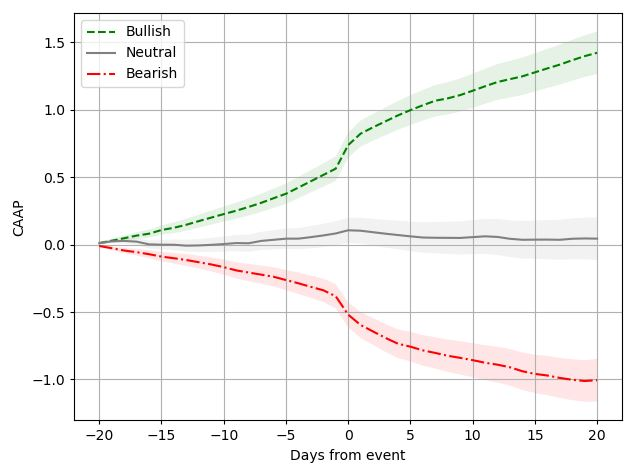
\includegraphics[width=0.75\textwidth]{caap.JPG}
    \mycaption{Cumulative average abnormal polarity around identified events.}{CAAP related to bearish, neutral and bullish events are displayed with the red, gray and green line, respectively. Areas around lines show confidence intervals at the 95\% level.}
    \label{fig:ES_cum_abn_pol_MM}
\end{figure}

\begin{figure*}[]
        \centering
        \begin{subfigure}[b]{0.42\textwidth}
            \centering
            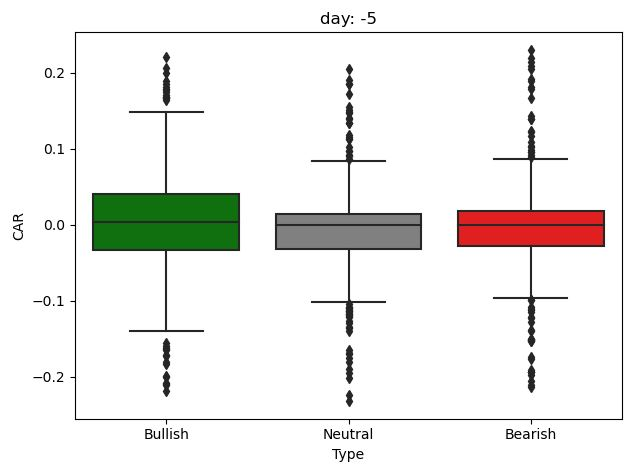
\includegraphics[width=\textwidth]{box_car_t-5.JPG}
            \caption*{CAR 5 days before the event}
        \end{subfigure}
        \quad
        \begin{subfigure}[b]{0.42\textwidth}  
            \centering 
            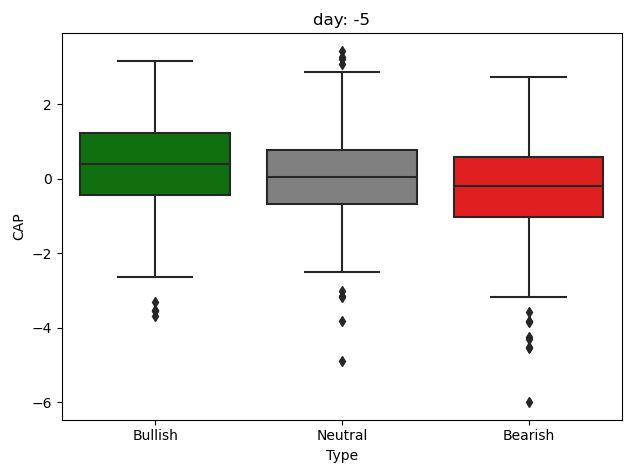
\includegraphics[width=\textwidth]{box_cap_t-5.JPG}
            \caption*{CAP 5 days before the event}  
        \end{subfigure}
        \vskip\baselineskip
        \begin{subfigure}[b]{0.42\textwidth}   
            \centering 
            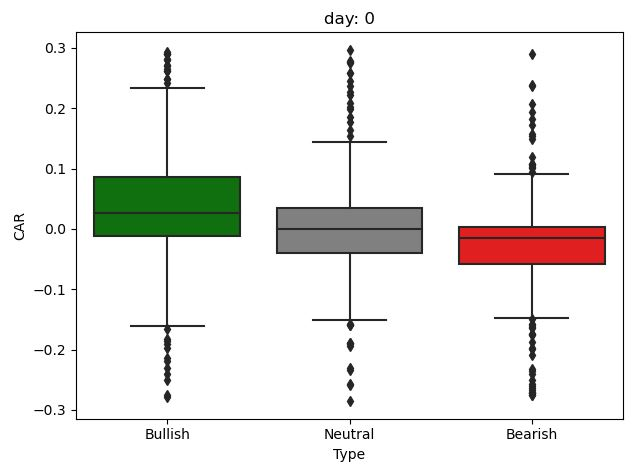
\includegraphics[width=\textwidth]{box_car_t.JPG}
            \caption*{CAR on the event date}   
        \end{subfigure}
        \quad
        \begin{subfigure}[b]{0.42\textwidth}   
            \centering 
            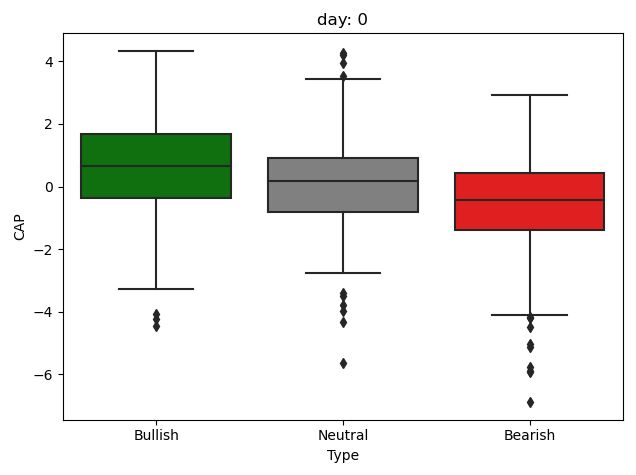
\includegraphics[width=\textwidth]{box_cap_t.JPG}
            \caption*{CAP on the event date}   
        \end{subfigure}
                \vskip\baselineskip
        \begin{subfigure}[b]{0.42\textwidth}   
            \centering 
            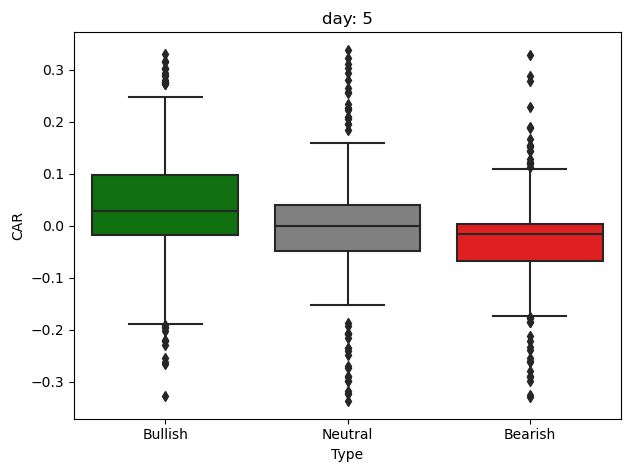
\includegraphics[width=\textwidth]{box_car_t+5.JPG}
            \caption*{CAR 5 days after the event}
        \end{subfigure}
        \quad
        \begin{subfigure}[b]{0.42\textwidth}   
            \centering 
            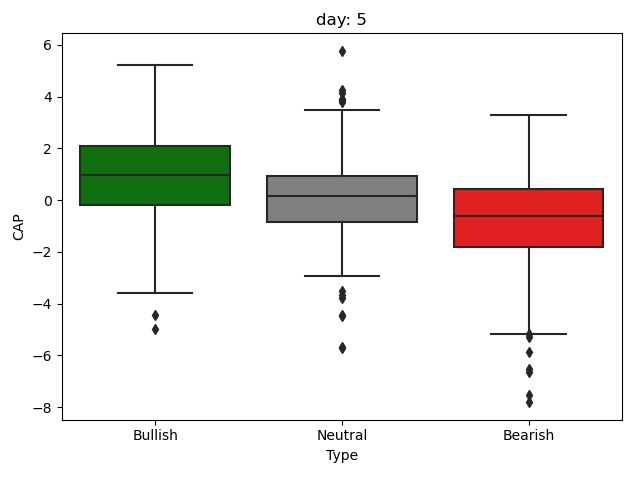
\includegraphics[width=\textwidth]{box_cap_t+5.JPG}
            \caption*{CAP 5 days after the event}  
        \end{subfigure}
        \mycaption{Distributions of CAP and CAR}{Distributions of CAP and CAR 5 days before an event, on event date and 5 days after an event. The line inside a box shows the median while the edges of each box represent the 25\% and 75\% quantile of the distribution. From the edges of a box, a distance of 1.5 times the interquartile range is measured and a whisker is drawn up to the largest and lowest observed point from the data that falls within this distance.} 
        \label{fig:boxplotcaar}
    \end{figure*}

% Please add the following required packages to your document preamble:
% \usepackage{multirow}
\begin{table}[]
\centering
\begin{tabular}{|c|c|c|c|c|c|}
\hline
\multicolumn{6}{|c|}{CAR}                                                                                                                                    \\ \hline 
\multicolumn{1}{|l|}{}                     & Alternative Hypothesis                                                         & U     & Z        & $n_1$ & $n_2$ \\ \hline
\multicolumn{1}{|l|}{\multirow{2}{*}{$\tau$-5}} & $H_1$ : $\theta_{bullish} > \theta_{neutral}$ & 61109 & -1.70    & 452  & 292  \\
\multicolumn{1}{|l|}{}                     & $H_1$ : $\theta_{neutral} > \theta_{bearish}$  & 54168 & -0.52    & 292  & 380  \\ \hline
\multirow{2}{*}{$\tau$}                         & $H_1$ : $\theta_{bullish} > \theta_{neutral}$ & 50967 & -5.25*** & 452  & 292  \\
                                           & $H_1$ : $\theta_{neutral} > \theta_{bearish}$  & 43100 & -4.96*** & 292  & 380  \\ \hline
\multirow{2}{*}{$\tau$+5}                       & $H_1$ : $\theta_{bullish} > \theta_{neutral}$ & 52738 & -4.63*** & 452  & 292  \\
                                           & $H_1$ : $\theta_{neutral} > \theta_{bearish}$  & 43239 & -4.91*** & 292  & 380  \\ \hline \hline
\multicolumn{6}{|c|}{CAP}                                                                                                                                    \\ \hline
\multicolumn{1}{|l|}{}                     & Alternative Hypothesis                                                         & U     & Z        & $n_1$ & $n_2$ \\ \hline
\multicolumn{1}{|l|}{\multirow{2}{*}{$\tau$-5}} & $H_1$ : $\theta_{bullish} > \theta_{neutral}$ & 55408 & -3.70*** & 452  & 292  \\
\multicolumn{1}{|l|}{}                     & $H_1$ : $\theta_{neutral} > \theta_{bearish}$  & 47998 & -3.00***   & 292  & 380  \\ \hline
\multirow{2}{*}{$\tau$}                         & $H_1$ : $\theta_{bullish} > \theta_{neutral}$ & 49385 & -8.98*** & 452  & 292  \\
                                           & $H_1$ : $\theta_{neutral} > \theta_{bearish}$  & 42101 & -5.36*** & 292  & 380  \\ \hline
\multirow{2}{*}{$\tau$+5}                       & $H_1$ : $\theta_{bullish} > \theta_{neutral}$ & 44364 & -7.55*** & 452  & 292  \\
                                           & $H_1$ : $\theta_{neutral} > \theta_{bearish}$  & 40515 & -6.00*** & 292  & 380  \\ \hline
\end{tabular}
\mycaption{Mann-Whitney U-test estimates}{Mann-Whitney U-test estimates for pairwise significant differences between distribution medians. Under the null hypothesis, the two samples represent two distributions with equal median values. Statistical significance at the 99\%, 95\%, and 90\% level is indicated with ***, **, *, respectively.}
\label{utest_res}
\end{table}

\section{Portfolios} \label{S:portfolios}

For the construction of a portfolio, in practice, we cannot condition on an event happening over the holding period. But we can repeat an experiment many times by supposing there is an event during the holding period and invest according to this hypothesis (long or short according to CAP). We would hope that repeating this experiment many times, we will be correct a few times and make large gain (or loss).

Our further intuition is that the larger the magnitude of $\mid$CAP$\mid$, the more likely there will be an event in the holding period. We have no statistical evidence for this, but intuitively, it makes sense to assume that the magnitude $\mid$CAP$\mid$ is a  “proxy” for predicting whether an event will happen or not. In that sense, we should better calibrate the thresholds such that the portfolio is zero quite often. Only if we have reason to believe that there will be an event (large magnitude $\mid$CAP$\mid$) then we invest, according to the sign of CAP. Otherwise we stay out of the market.

The data consists of ticker-date instances $(i,t)$, for the universe of tickers $i=1,\dots,19$ and dates $t$ ranging through all business days of the sample period, excluding the first 14 days (for the CAP) and the last day (for the last holding period). Every ticker-date instance $(i,t)$ comes with the feature $CAP_{i,t}=\sum_{s=t-14}^t AP_{i,s}$, which is the running CAP over the last 14 days plus current day $t$ (we do end of day $t$ rebalancing). Note this is different from the definition of ``$CAP_i(\tau,t)$'' above.
    
   % \item label $L_{it}$, taking 4 categorical values:
   % \[ L_{i,t}=\begin{cases} \text{bullish},&\text{if there is a %bullish event of ticker $i$ during $t+1,\dots,t+5$,}\\ %\text{neutral},&\text{if there is a neutral event of ticker $i$ %during $t+1,\dots,t+5$,}\\ \text{no},&\text{if there is no event %of ticker $i$ during $t+1,\dots,t+5$,}\\ \text{bearish},&\text{if %there is a bearish event of ticker $i$ during %$t+1,\dots,t+5$}\end{cases}\]


\subsection{CAP reset after an event}

As CAP continues to shift after an event, for our portfolio construction, we chose to reset it to 0 after every event. This ensures that we are not exposed to short-term reversals. Let $CAP_{i,t}^{(R)}$ be the feature time-serie of the CAP reset to 0 after every event. Formally, let $\tau_{i,t}\le t$ denote the most recent past event date by $t$ of ticker $i$. Then we define
\[ CAP_{i,t}^{(R)} = \sum_{s=\max\{t-14,\tau_{i,t}+1\}}^t AP_{i,s} = \begin{cases} CAP_{i,t},&\text{if $\tau_{i,t}<t-14$,} \\ \sum_{s= \tau_{i,t}+1}^t AP_{i,s},&\text{if $t-14\le \tau_{i,t}<t$,}\\
0,&\text{if $\tau_{i,t}=t$,}\end{cases}\]
where we used the convention that $\sum_{s=t+1}^t \cdot =0$.

\subsection{Cross-sectional thresholds}

We use time-varying thresholds to build a long and a short portfolio. For every day, we compute the cross-sectional mean and standard deviations of  $CAP_{i,t}^{(R)}$ across the 19 tickers. We will use the mean $\pm$ $x$ standard deviations as and up and down thresholds in the portfolio construction, with $x$ as hyperparameter. We define $U_t(x) = \mu_t + x \cdot \sigma_t$ the upper threshold, and $L_t(x) = \mu_t - x \cdot \sigma_t$ the lower threshold, with $\mu_t$ and $\sigma_t$ being the cross-sectional mean and standard deviations, respectively.  Figure \ref{fig:cross-sec stats} shows the cross-sectional mean and its 99\% confidence interval ($x$ = 2.58). The mean is well centered at zero, which speaks for our method of computing CAP. It also shows that there are essentially two regimes, with a switch in early 2015. In the first regime the standard deviation is much larger (and more volatile) than in the second regime. The Appendix contains the results for 95\% ($x$ = 1.96) and 99.5\% confidence intervals ($x$ = 2.81). 

\begin{figure}
    \centering
    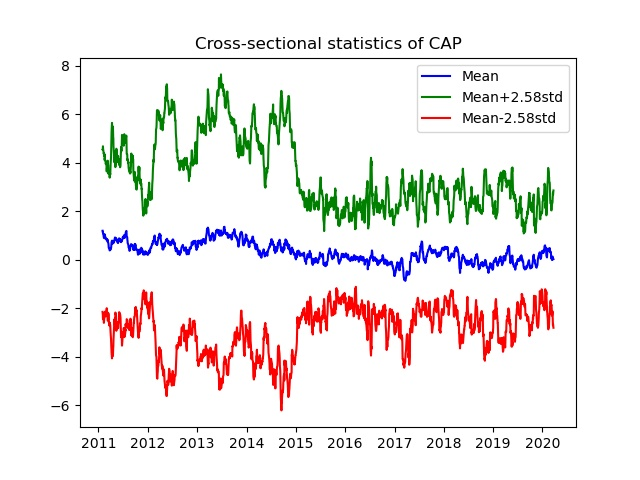
\includegraphics[width=0.75\textwidth]{cross_sectional_cap.jpg}
    \mycaption{Cross-sectional statistics of $CAP^{(R)}$.}{The blue lines shows the cross-sectional mean of the CAP across the 19 tickers over the year. The green and red lines show the up and down 99\% confidence band. We use them as up and down thresholds for the portfolio construction. }
    \label{fig:cross-sec stats}
\end{figure}


%\subsection{Long/not-long classification}
%
%We want to learn the binary label
%
%\[ L^{long}_{i,t} = \begin{cases} \text{long}, &\text{if %$L_{i,t}=\text{bullish}$,}\\\text{not-long}, &\text{if %$L_{i,t}\in\{\text{neutral},\text{no},\text{bearish}\}$,} \end{cases}
%\]
%Thereto, we choose a threshold $c^{long}$ and predict $\hat %L^{long}_{i,t}=\text{long}$ if $CAP_{i,t}^{(R)}>c^{long}$.
%
%Doing so gives a $2\times 2$ confusion matrix 
%
%\begin{table}[H]
%\centering
%\begin{tabular}{c|c|c|}
%predicted label & \multicolumn{2}{c|}{true label}  \\ \hline
% & long & not-long \\ \hline
%  long &  TP & FP \\\hline
%  not-long & FN & TN
%\end{tabular}
%\end{table}
%
%(this table can be better plotted than here)
%
%Compute precision, recall, F1-score, or the Matthews Correlation Coefficient %MCC (see \url{https://en.wikipedia.org/wiki/Phi_coefficient#Confusion_matrix})
% 
%Then find $c^{long}$ that maximizes F1-score or MCC
%
%
%\subsection{Short/not-short classification}
%
%We want to learn the binary label
%
%\[ L^{short}_{i,t} = \begin{cases} \text{short}, &\text{if %$L_{i,t}=\text{bearish}$,}\\\text{not-short}, &\text{if %$L_{i,t}\in\{\text{bullish},\text{neutral},\text{no}\}$,} \end{cases}
%\]
%Thereto, we choose a threshold $c^{short}$ and predict $\hat %L^{short}_{i,t}=\text{short}$ if $CAP_{i,t}^{(R)}<c^{short}$.
%
%Doing so gives a $2\times 2$ confusion matrix 
%
%\begin{table}[H]
%\centering
%\begin{tabular}{c|c|c|}
%predicted label & \multicolumn{2}{c|}{true label}  \\ \hline
% & short & not-short \\ \hline
%  short &  TP & FP \\\hline
%  not-short & FN & TN
%\end{tabular}
%\end{table}
%
%(this table can be better plotted than here)
%
%Compute precision, recall, F1-score, or the Matthews Correlation Coefficient %MCC (see \url{https://en.wikipedia.org/wiki/Phi_coefficient#Confusion_matrix})
% 
%Then find $c^{short}$ that maximizes F1-score or MCC


\subsection{Portfolio and returns}

We look at two types of portfolios: long only, and short only that we hold for one day.

Denote by $R_{i,t+1}=(S_{i,t+1}-S_{i,t})/S_{i,t} - R_{f,t}$ the excess return of ticker $i$ over $[t,t+1]$. 

\paragraph{Long only:}

At the end of any business day $t$, we go long all tickers $i$ with $CAP_{i,t}^{(R)} > U_t(x)$. Denote by $I^{long}_t=\{ i\mid CAP_{i,t}^{(R)} > U_t(x)\}$ the corresponding index set, which could be empty. We then form an equally weighted portfolio and consider the 1-day excess return
\[ R^{long}_{t,t+1} = \begin{cases} \frac{1}{|I^{long}_t|}\sum_{i\in I^{long}_t} R_{i,t,t+1} ,&\text{if $I^{long}_t\neq \emptyset$.} \\
0, &\text{if $I^{long}_t = \emptyset$.} \end{cases}\]


\paragraph{Short only:}

At the end of any business day $t$, we go long all tickers $i$ with $CAP_{i,t}^{(R)} < L_t(x)$. Denote by $I^{short}_t=\{ i\mid CAP_{i,t}^{(R)} < L_t(x)\}$ the corresponding index set, which could be empty. We then form an equally weighted portfolio and consider the 1-day excess return
\[ R^{short}_{t,t+1} = \begin{cases} \frac{1}{|I^{short}_t|}\sum_{i\in I^{short}_t} R_{i,t,t+1} ,&\text{if $I^{short}_t\neq \emptyset$.} \\
0, &\text{if $I^{short}_t = \emptyset$.} \end{cases}\]


Now, we compute these returns for all $t$ and plot a time series.  What we would like to see, of course, is significantly positive excess returns $R^{long}_{t,t+1}$ and negative excess returns $R^{short}_{t,t+1}$. 

Figure \ref{fig:cumretpf} shows the cumulative log returns of long and short portfolios as well as the S\&P500. Overall, the strategies are correct in both direction : the long portfolio shows positive returns and the short portfolio shows negative returns. Remarkably, cumulative log returns are most of the time shaped as step functions, suggesting that the strategy is able to take positions before an event, and close the position after the return is earned due to the CAP reset. Figure \ref{fig:pf} shows the number of positions across time of our portfolios. Most of the returns are earned with portfolios consisting of very few tickers. This is a result of our stock picking strategy : we only invest in the top/bottom percentile of CAP, whenever possible.

\begin{figure}
    \centering
    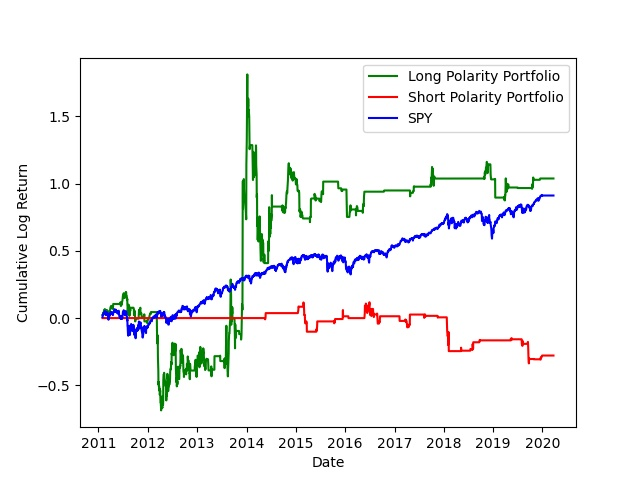
\includegraphics[width=0.75\textwidth]{cumulative_log_return.jpg}
    \mycaption{Cumulative log returns of both portfolios (x=2.58) and the S\&P500.}{}
    \label{fig:cumretpf}
\end{figure}

\begin{figure*}[]
        \centering
        %\begin{subfigure}[b]{0.42\textwidth}
        %    \centering
        %    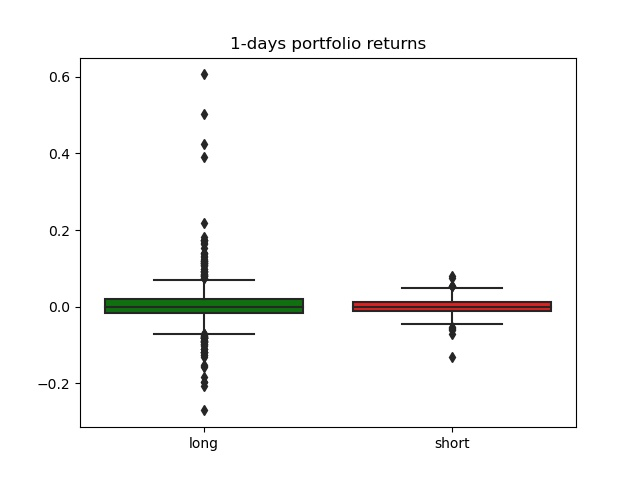
\includegraphics[width=\textwidth]{boxplot.JPG%}
        %    \caption*{Distribution of returns}
        %\end{subfigure}
        %\quad
        %\begin{subfigure}[b]{0.42\textwidth}  
        %    \centering 
        %    \includegraphics[width=\textwidth]{boxplot_zoo%med.JPG}
        %    \caption*{Distribution of returns - zoomed}  
        %\end{subfigure}
        %\vskip\baselineskip
        \begin{subfigure}[b]{0.42\textwidth}   
            \centering 
            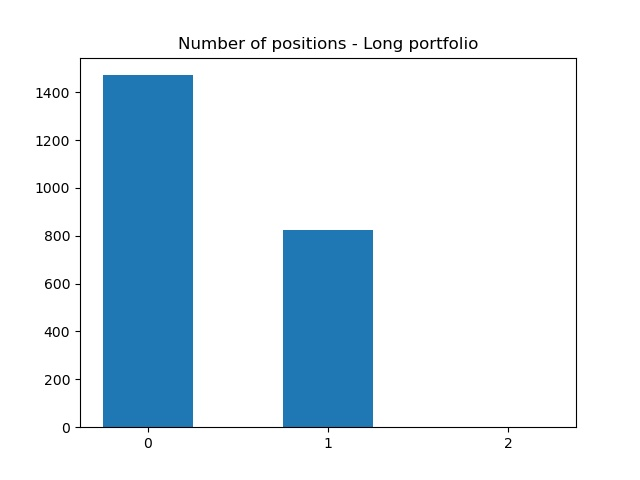
\includegraphics[width=\textwidth]{distribution_long_positions.JPG}
            \caption*{Number of positions - Long portfolio}   
        \end{subfigure}
        \quad
        \begin{subfigure}[b]{0.42\textwidth}   
            \centering 
            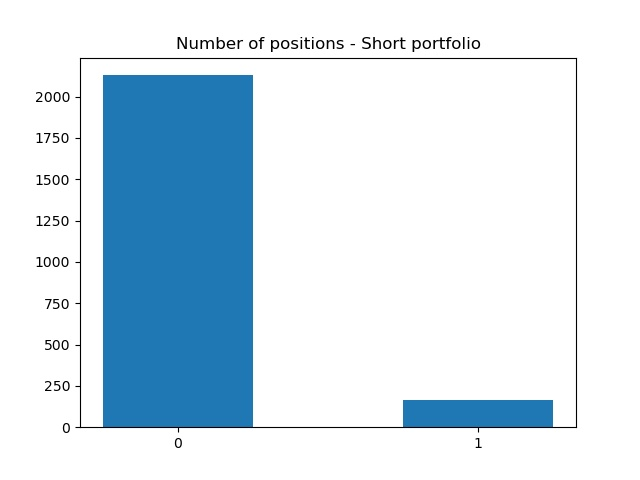
\includegraphics[width=\textwidth]{distribution_short_positions.JPG}
            \caption*{Number of positions - Short portfolio}   
        \end{subfigure}
                \vskip\baselineskip
        \begin{subfigure}[b]{0.42\textwidth}   
            \centering 
            \includegraphics[width=\textwidth]{positions.JPG}
            \caption*{Number of positions over time}
        \end{subfigure}
        \quad
        \begin{subfigure}[b]{0.42\textwidth}   
            \centering 
            \includegraphics[width=\textwidth]{returns.JPG}
            \caption*{Daily returns}  
        \end{subfigure}
        \mycaption{Long and Short portfolios for x=2.58.}{}
        \label{fig:pf}
    \end{figure*}




%\input{drawdowns}
\newpage
\section{Conclusion} \label{S:conclusion}

We believe that an accurate and timely estimation of investor sentiment on both firms and aggregate market is an excellent proxy of unobservable firm fundamentals. In particular, recent studies on \textit{nowcasting} shows that alternative sources of data can enhance traditional models of stock return and accounting earnings predictions (\citet{challet2013predicting}). In this paper, we scrape 90 million messages out of StockTwits during 2010 to 2020. Messages are either user-labeled as bullish or bearish or left unlabeled. Using the labeled messages as training set, we build a logistic regression on TFIDF vectorized messages to classify the unlabeled messages in either bullish, neutral or bearish class. We observe a 5-for-1 bullish-to-bearish ratio, indicating that investors are on average optimistic. Then, we build daily time-series of polarity for both individual firms and the aggregate market. We show that changes in daily polarity are strongly associated to changes of the same sign in contemporaneous stock returns, but this result loses its significance against next-day returns. However, focused around specific firm events (defined as sudden peak of message volume on a firm), we show that cumulative abnormal polarity has much more predictive power than cumulative abnormal returns. We also note that user's sentiment about a firm tend to be biased towards recent past events. Finally, as robustness check, we show that event studies on CAAR are consistent with previous literature on EMH.

